\documentclass{beamer}
\setbeamertemplate{navigation symbols}{}
\usepackage{graphics}
\usepackage{amsmath}
\usetheme{Warsaw}
%\usepackage{url}
%\usepackage{cite}
\usepackage{multirow}
\beamersetuncovermixins{\opaqueness<1>{25}}{\opaqueness<2->{1}}
\begin{document}
\title{Word Search Puzzle (P9)}  
\author{Venkhat V, Pinkesh Barsopia}
\titlegraphic{\includegraphics[scale=0.2]{iitblogo.jpg}}
\institute{Department of Electrical Engineering\\ Indian Institute of Technology Bombay\\ Guide: Prof. Abhay Karandikar}
\date{May 6, 2013} 


%\begin{frame}
%\titlepage
%\end{frame}
%\begin{frame}[shrink]\frametitle{Outline}
%\tableofcontents
%\end{frame} 



\begin{frame}\frametitle{Word Search Puzzle (P9) - Project Aim }
\begin{itemize}
 \item Interactive game based on Classic Word Search Puzzle
\item Search a set of words embedded in a $N \times N$ matrix of characters

\end{itemize}
\begin{columns}[c]
\begin{column}{5cm}
Different features
\begin{enumerate}
\item User selectable difficulty levels and Grid Size
\item Score
\item Time limit
\end{enumerate}
\end{column}
\begin{column}{5cm}

\begin{figure}
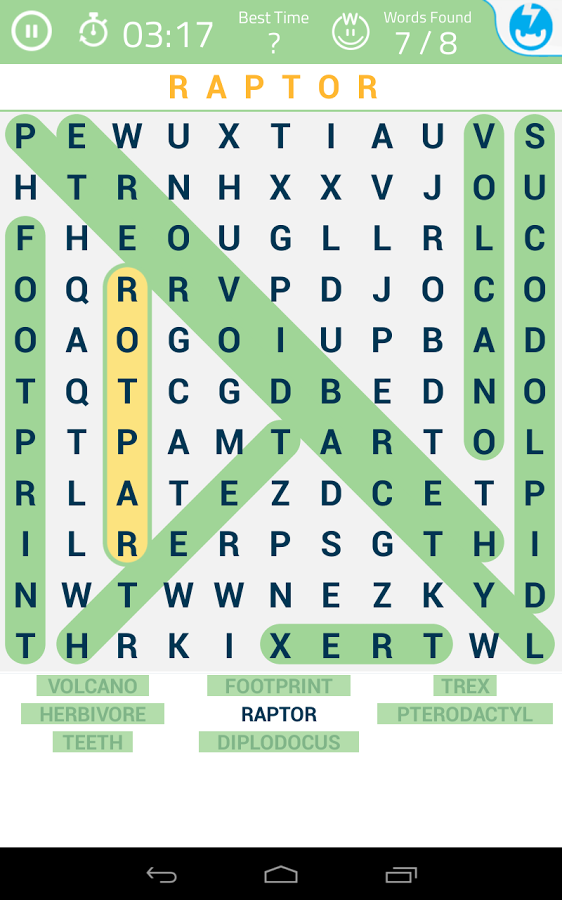
\includegraphics[scale=0.15]{word_puzzle.png}
\end{figure}
\end{column}
\end{columns}
\end{frame}

\begin{frame}\frametitle{Game Specifications}
\begin{columns}[c]
\begin{column}{5cm}

\textbf{User Input }
\begin{enumerate}
\item Size of grid - N
\item Difficulty level - Easy, Medium Hard

\end{enumerate}
\end{column}
\begin{column}{5cm}
\textbf{Game parameters}
\begin{enumerate}
\item Length of longest word, L
\item Intersection of words, I
\item Display the set of words  
\item Random filling of characters
\end{enumerate}
\end{column}
\end{columns}

%\begin{table}[h!] 
\centering
%\capti\on{}
\label{tablewc}
\resizebox{\columnwidth}{!}
{

\begin{tabular}{|c|l | l | l |}
\hline
 & Level 1 & Level  2 & Level 3 \\
\hline
  & I- No & I- Yes & I- Yes\\
& Display - Yes & Display - Yes & Display - Yes  \\ \hline
\multirow{2}{*}{N = 10}  & WL - 4 &  WL- 5 & WL - 5\\
& No.of words =5 & No. of words =8 & No. of words =10\\
\hline
\multirow{2}{*}{N = 15}  & WL - 6 &  WL- 8 & WL - 8\\
& No.of words =10 & No. of words =15 & No. of words =20\\
\hline
\end{tabular}
}
\vfill
\textbf{PyGame- GUI , Python - algorithm}
%\end{table} 
\end{frame}

\begin{frame}\frametitle {Brief outline of work completed till now}
\textbf{Modules}
\begin{itemize} 
\item \textbf{charmat} - holds matrix and get and set word and random fill function
\item \textbf{wordlist}
\begin{itemize} \item holds word list and strategically populates matrix with words  \item  chooses words and places them according to the difficulty levels \end{itemize}
\item \textbf{GUI} - setting GUI parameters like size, colours, shapes etc
\end{itemize}
\textbf{Work Done}
\begin{itemize}
\item Completed above 3 modules with unit testing
\item Difficulty level 1 - ensuring no overlaps and even spread of words
\item GUI with fixed sized window, 2 mouse clicks selects the word  
 \end{itemize}
\end{frame}

\begin{frame}
\frametitle{Brief outline of work to be done in future}
Remaining Modules 
\begin{itemize}
\item \textbf{gamestatus} - holding current status, score, found words,  check validity of user selection
\item \textbf{main} - uses above modules along with GUI and runs the game
\end{itemize}
Work Remaining
\begin{itemize}

\item To complete above two modules
\item Build more features in GUI like resizing window, drag and select feature, user selectable options, sounds etc..
\item adding more difficulty level with controlled overlap etc..

\end{itemize}

\end{frame}

\end{document}